\begin{egBox}{Metric Topology}[eg:12-1]
    A metric space has an induced topology that we call the 
    \textbf{metric topology}.
    Notice that the condition for openness in this topology is determined 
    by the metric; e.g., \( \mathbb{R}^{ 2 } \) with the euclidean metric
    has the condition of openness via open balls.
\end{egBox}

\begin{egBox}{The Standard Topology on \( \mathbb{R} \)}[eg:12-2]
    Let \( X = \mathbb{R} \), and let \( \mathcal{T} \) to be all unions of 
    open intervals. We have that \( \mathcal{T} \) is a topology.

    \baseSkip

    To show why, it is clear that \( \emptyset \) and \( \mathbb{R} \) are in 
    \( \mathcal{T} \). 
    Furthermore, it is clear that \( \mathcal{T} \) is closed under unions since it follows by construction. 
    All that is left to do is to show that
    \( \mathcal{T} \) is closed under finite intersections.

    \baseSkip

    Take \( I_{ 1 }, \ldots, I_{ n } \in \mathcal{T} \). Note that \( I_{ 1 } 
    \cap I_{ 2 } \) is still an open interval (where
    we are taking \( \emptyset \) to be open), thus it follows by induction 
    that \( I_{ 1 } \cap \ldots \cap I_{ n } \) is still
    an open interval as well. Since we have \( \mathcal{T} \) to be all unions 
    of open intervals, it follows that
    \( I_{ 1 } \cap \ldots \cap I_{ n } \in \mathcal{T} \).

    \baseSkip

    We give this topology on \( \mathbb{R} \) a special name -- it is called 
    the \textbf{standard topology} on \( \mathbb{R} \).
\end{egBox}

\begin{egBox}{Discrete Topology}[eg:12-3]
    Let \( X \) be any set. The collection of \textit{all} subsets of \( X \) 
    is a topology on \( X \) -- called the \textbf{discrete topology}.

    \baseSkip

    To show why, we have right away that \( \emptyset \) and \( X \) are in 
    \( \mathcal{T} \) since both
    \( \emptyset, X \subset X \). 
    Furthermore, the second condition is met right away as well since the union 
    of any subcollection of \( \mathcal{T} \) is still a subset of \( X \). 
    All that is left to do is to show that \( \mathcal{T} \) is closed under 
    finite intersections.

    \baseSkip

    Take \( U_{ 1 }, \ldots, U_{ n } \in \mathcal{T} \). Notice that \( U_{ 1 } \cap \ldots \cap U_{ n } \) is a subset of each
    of the sets \( U_{ 1 }, \ldots, U_{ n } \) (this can be proved rigorously via induction), which are themselves subsets of
    \( X \). Hence it follows that \( U_{ 1 } \cap \ldots \cap U_{ n } \) is a subset of \( X \), which means that
    \( U_{ 1 } \cap \ldots \cap U_{ n } \in \mathcal{T} \).
\end{egBox}

\begin{egBox}{Trivial Topology}[eg:12-4]
    Let \( X \) be any set. The collection consisting of \( X \) and \( \emptyset \) only is a topology on \( X \) -- called the
    \textbf{indiscrete topology}, or the \textbf{trivial topology}. This is clear to see as \( \mathcal{T} \) consists of
    \( X \) and \( \emptyset \) only, which immediately results in the three conditions to be met.
\end{egBox}

\begin{egBox}{Finite Complement Topology}[eg:12-5]
    Let \( X \) be a set, and let \( \mathcal{T}_{ f } \) be the collection of 
    all subsets \( U \) of \( X \) such that \( X \setminus U \) is either 
    finite or is all of \( X \). 
    It follows that \( \mathcal{T}_{ f } \) is a topology on \( X \),
    called the \textbf{finite complement topology}.

    \baseSkip

    To show why, it is clear to see that both \( X \) and \( \emptyset \) are 
    in \( \mathcal{T}_{ f } \);
    \( X \setminus X = \emptyset \) is finite and 
    \( X \setminus \emptyset = X \) is all of \( X \).

    \baseSkip

    Let us now take
    \( \{ U_{ i } \}_{ i \in I } \) to be an indexed family of 
    nonempty elements of \( \mathcal{T}_{ f } \). Our
    goal is to show that 
    \( \bigcup_{ i \in I } U_{ i } \in \mathcal{T}_{ f } \), which just 
    amounts to showing that
    \( X \setminus \bigcup_{ i \in I } U_{ i } \) is finite. 
    Notice that DeMorgan's law tells us
    \begin{equation*}
        X \setminus \bigcup_{ i \in I } U_{ i } 
        = 
        \bigcap_{ i } ( X \setminus U_{ i } )
    \end{equation*}
    Because we have each \( U_{ i } \in \mathcal{T} \), it follows that \( X 
    \setminus U_{ i } \) is finite by construction.
    Thus, we
    have that \( \bigcap_{ i \in I } ( X \setminus U_{ i } ) \) is finite as 
    arbitrary intersections of finite sets are finite,
    which takes care of the second condition.

    \baseSkip
    
    Let us now take \( U_{ 1 }, \ldots, U_{ n } \) to be a finite collection of 
    nonempty elements of \( \mathcal{T}_{ f } \).
    We want to show that \( U_{ 1 } \cap \ldots \cap U_{ n } \in 
    \mathcal{T}_{ f } \). Again, this just amounts to showing that
    \( X \setminus U_{ 1 } \cap \ldots \cap U_{ n } \) is finite. In this case, 
    DeMorgan's law tells us
    \begin{equation*}
        X \setminus U_{ 1 } \cap \ldots \cap U_{ n }
        =
        \bigcup_{ i = 1 }^{ n } ( X \setminus U_{ i } )
    \end{equation*}
    Since we know from above that \( X \setminus U_{ i } \) is finite, we have 
    that \( \bigcup_{ i = 1 }^{ n } ( X \setminus U_{ i } ) \)
    is finite as a finite union of finite sets is still finite. This finishes 
    the proof.
\end{egBox}

\begin{egBox}{Countable Complement Topology}[eg:12-6]
    Let \( X \) be a set, and let \( \mathcal{T}_{ c } \) be the collection of all subsets \( U \) of \( X \) such that
    \( X \setminus U \) is either countable or is all of \( X \). It follows that \( \mathcal{T}_{ c } \) is a topology on \( X \).

    \baseSkip

    To show why, it is clear to see that both \( X \) and \( \emptyset \) are 
    in \( \mathcal{T}_{ c } \);
    \( X \setminus X = \emptyset \) is finite (which is countable) and \( X 
    \setminus \emptyset = X \) is all of \( X \).

    \baseSkip

    Let us now take
    \( \{ U_{ i } \}_{ i \in I } \) to be an indexed family of nonempty 
    elements of \( \mathcal{T}_{ c } \). Our
    goal is to show that \( \bigcup_{ i \in I } U_{ i } \in 
    \mathcal{T}_{ c } \), which just amounts to showing that
    \( X \setminus \bigcup_{ i \in I } U_{ i } \) is countable. Notice that 
    DeMorgan's law tells us
    \begin{equation*}
        X \setminus \bigcup_{ i \in I } U_{ i } 
        = 
        \bigcap_{ i \in I } ( X \setminus U_{ i } )
    \end{equation*}
    Because we have each \( U_{ i } \in \mathcal{T} \), it follows that \( X 
    \setminus U_{ i } \) is countable by
    construction. Thus, we
    have that \( \bigcap_{ i \in I } ( X \setminus U_{ i } ) \) is countable as 
    arbitrary intersections of countable sets are still
    countable; such a statement is true by noting that \( \bigcap_{ i \in I } 
    ( X \setminus U_{ i } ) \) is a subset of all
    \( \{ U_{ i } \}_{ i \in I } \), and a subset of a countable set is still 
    countable.

    \baseSkip

    Let us now take \( U_{ 1 }, \ldots, U_{ n } \) to be a finite collection of 
    nonempty elements of \( \mathcal{T}_{ c } \).
    We want to show that \( U_{ 1 } \cap \ldots \cap U_{ n } \in 
    \mathcal{T}_{ c } \). Again, this just amounts to showing that
    \( X \setminus U_{ 1 } \cap \ldots \cap U_{ n } \) is countable. In this 
    case, DeMorgan's law tells us
    \begin{equation*}
        X \setminus U_{ 1 } \cap \ldots \cap U_{ n }
        =
        \bigcup_{ i = 1 }^{ n } ( X \setminus U_{ i } )
    \end{equation*}
    Since we know from above that \( X \setminus U_{ i } \) is countable, we 
    have that \( \bigcup_{ i = 1 }^{ n } ( X \setminus U_{ i } ) \)
    is countable as a finite (in fact, we can have a countable amount) union of 
    countable sets is still countable.
    This finishes the proof.
\end{egBox}

\begin{egBox}{Topology of a 3-element Set}[eg:12-7]
    Let \( X \) be a three-element set, \( X = \{ a, b, c \} \). There are 
    many possible topologies on \( X \) -- a few of which are shown in 
    Figure \ref{fig:12_3elem1}. 
    Notice that the diagram in the upper left-hand corner indicates the trivial 
    topology, and the diagram in the lowe right-hand corner indicates the 
    discrete topology.
    \begin{figure}[H]
        \centering
        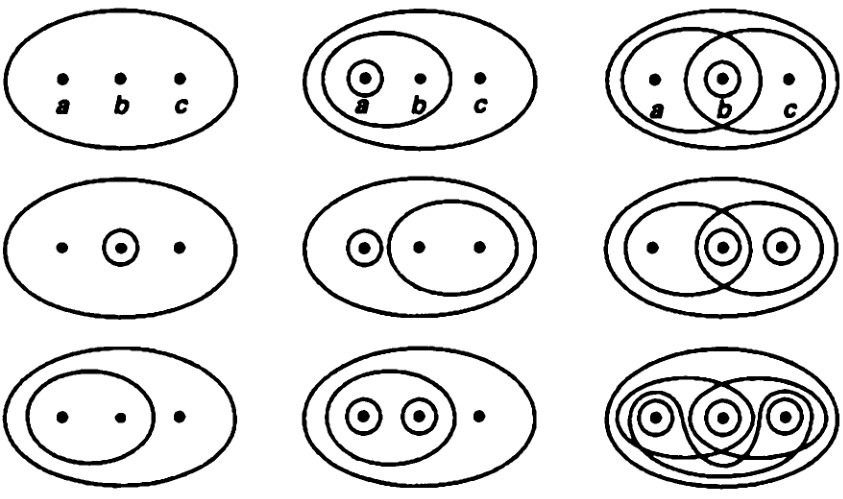
\includegraphics[ width = 0.5\linewidth ]{figures/Section 12/eg1.jpg}
        \caption{Some Possible Topologies on \( X \)}
        \label{fig:12_3elem1}
    \end{figure}
    The two diagrams shown in Figure \ref{fig:12_3elem2} are examples of 
    non-topologies in \( X \).
    \begin{figure}[H]
        \centering
        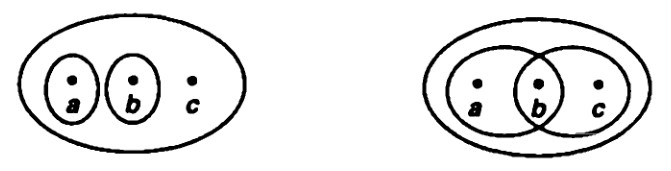
\includegraphics[ width = 0.5\linewidth ]{figures/Section 12/eg2.jpg}
        \caption{Some Possible Non-Topologies on \( X \)}
        \label{fig:12_3elem2}
    \end{figure}
    The left diagram is not a topology because it is not closed under arbitrary 
    unions, and the right diagram is not a topology because it is not closed 
    under finite intersections.
\end{egBox}

\begin{egBox}{Comparing Topologies on \( \mathbb{R} \)}[eg:12-8]
    Let \( X = \mathbb{R} \). Compare the following topologies on 
    \( \mathbb{R} \):
    \begin{equation*}
        \mathcal{T}_{ \mathrm{discrete} },
        \mathcal{T}_{ \mathrm{trivial} },
        \mathcal{T}_{ \mathrm{standard} },
        \mathcal{T}_{ \mathrm{cofinite} }
    \end{equation*}
    Here the standard topology on \( \mathbb{R} \) means the same thing as the 
    Euclidean topology. 

    \baseSkip

    We see that 
    \begin{equation*}
        \mathcal{T}_{ \mathrm{trivial} }
        \subset
        \mathcal{T}_{ \mathrm{cofinite} }
        \subset
        \mathcal{T}_{ \mathrm{standard} }
        \subset
        \mathcal{T}_{ \mathrm{discrete} }
    \end{equation*}
    One can immediately expect \( \mathcal{T}_{ \mathrm{trivial} } \) and 
    \( \mathcal{T}_{ \mathrm{discrete} } \) to be the coarsest and finest
    topologies, respectively.
    This leaves us with finding where \( \mathcal{T}_{ \mathrm{cofinite} } \) 
    and \( \mathcal{T}_{ \mathrm{standard} } \) should be placed inclusion-wise.

    \baseSkip

    We can immediately see that for any open interval \( ( a, b ) \) in 
    \( \mathcal{T}_{ \mathrm{standard} } \), we see that its complement 
    is not finite -- thus, we have that \( \mathcal{T}_{ \mathrm{cofinite} } \)
    cannot contain \( \mathcal{T}_{ \mathrm{standard} } \).
    We now want to see whether \( \mathcal{T}_{ \mathrm{standard} } \) contains
    \( \mathcal{T}_{ \mathrm{cofinite} } \).
    This amounts to showing that every open set in 
    \( \mathcal{T}_{ \mathrm{cofinite} } \) is also open in 
    \( \mathcal{T}_{ \mathrm{standard} } \).

    \baseSkip

    Let \( U \) be any open set in \( \mathcal{T}_{ \mathrm{cofinite} } \).
    By definition, this means that \( \mathbb{R} \setminus U \) is either 
    finite or the \( \emptyset \).
    Assuming that it is finite (the \( \emptyset \) is trivially open in any
    topology), we have that
    \begin{equation*}
        \mathbb{R} \setminus U
        =
        \{ x_{ 1 } , \ldots , x_{ n } \}
        \quad \mathrm{where} \quad 
        n \in \mathbb{Z}_{ + }
    \end{equation*}
    Furthermore, let us assume that the finite point set is ordered from 
    smallest to largest -- that is, \( x_{ 1 } \leq \ldots \leq x_{ n } \).
    With this, we see that \( U \) must be of the following form:
    \begin{equation*}
        U
        =
        ( - \infty, x_{ 1 } ) \cup ( x_{ 1 }, x_{ 2 } ) 
        \cup \ldots \cup 
        ( x_{ n - 1 }, x_{ n } ) \cup ( x_{ n }, \infty )
    \end{equation*}
    which is just a union of open intervals, which is also open itself.
    Thus, \( U \) is open in \( \mathcal{T}_{ \mathrm{standard} } \) as well.

    \baseSkip

    As a result, we are left with \( \mathcal{T}_{ \mathrm{cofinite} } \subset
    \mathcal{T}_{ \mathrm{standard} } \).
\end{egBox}